\begin{figure}[!ht]
    \subfloat[\label{fig:so_pix_size:a}]{
        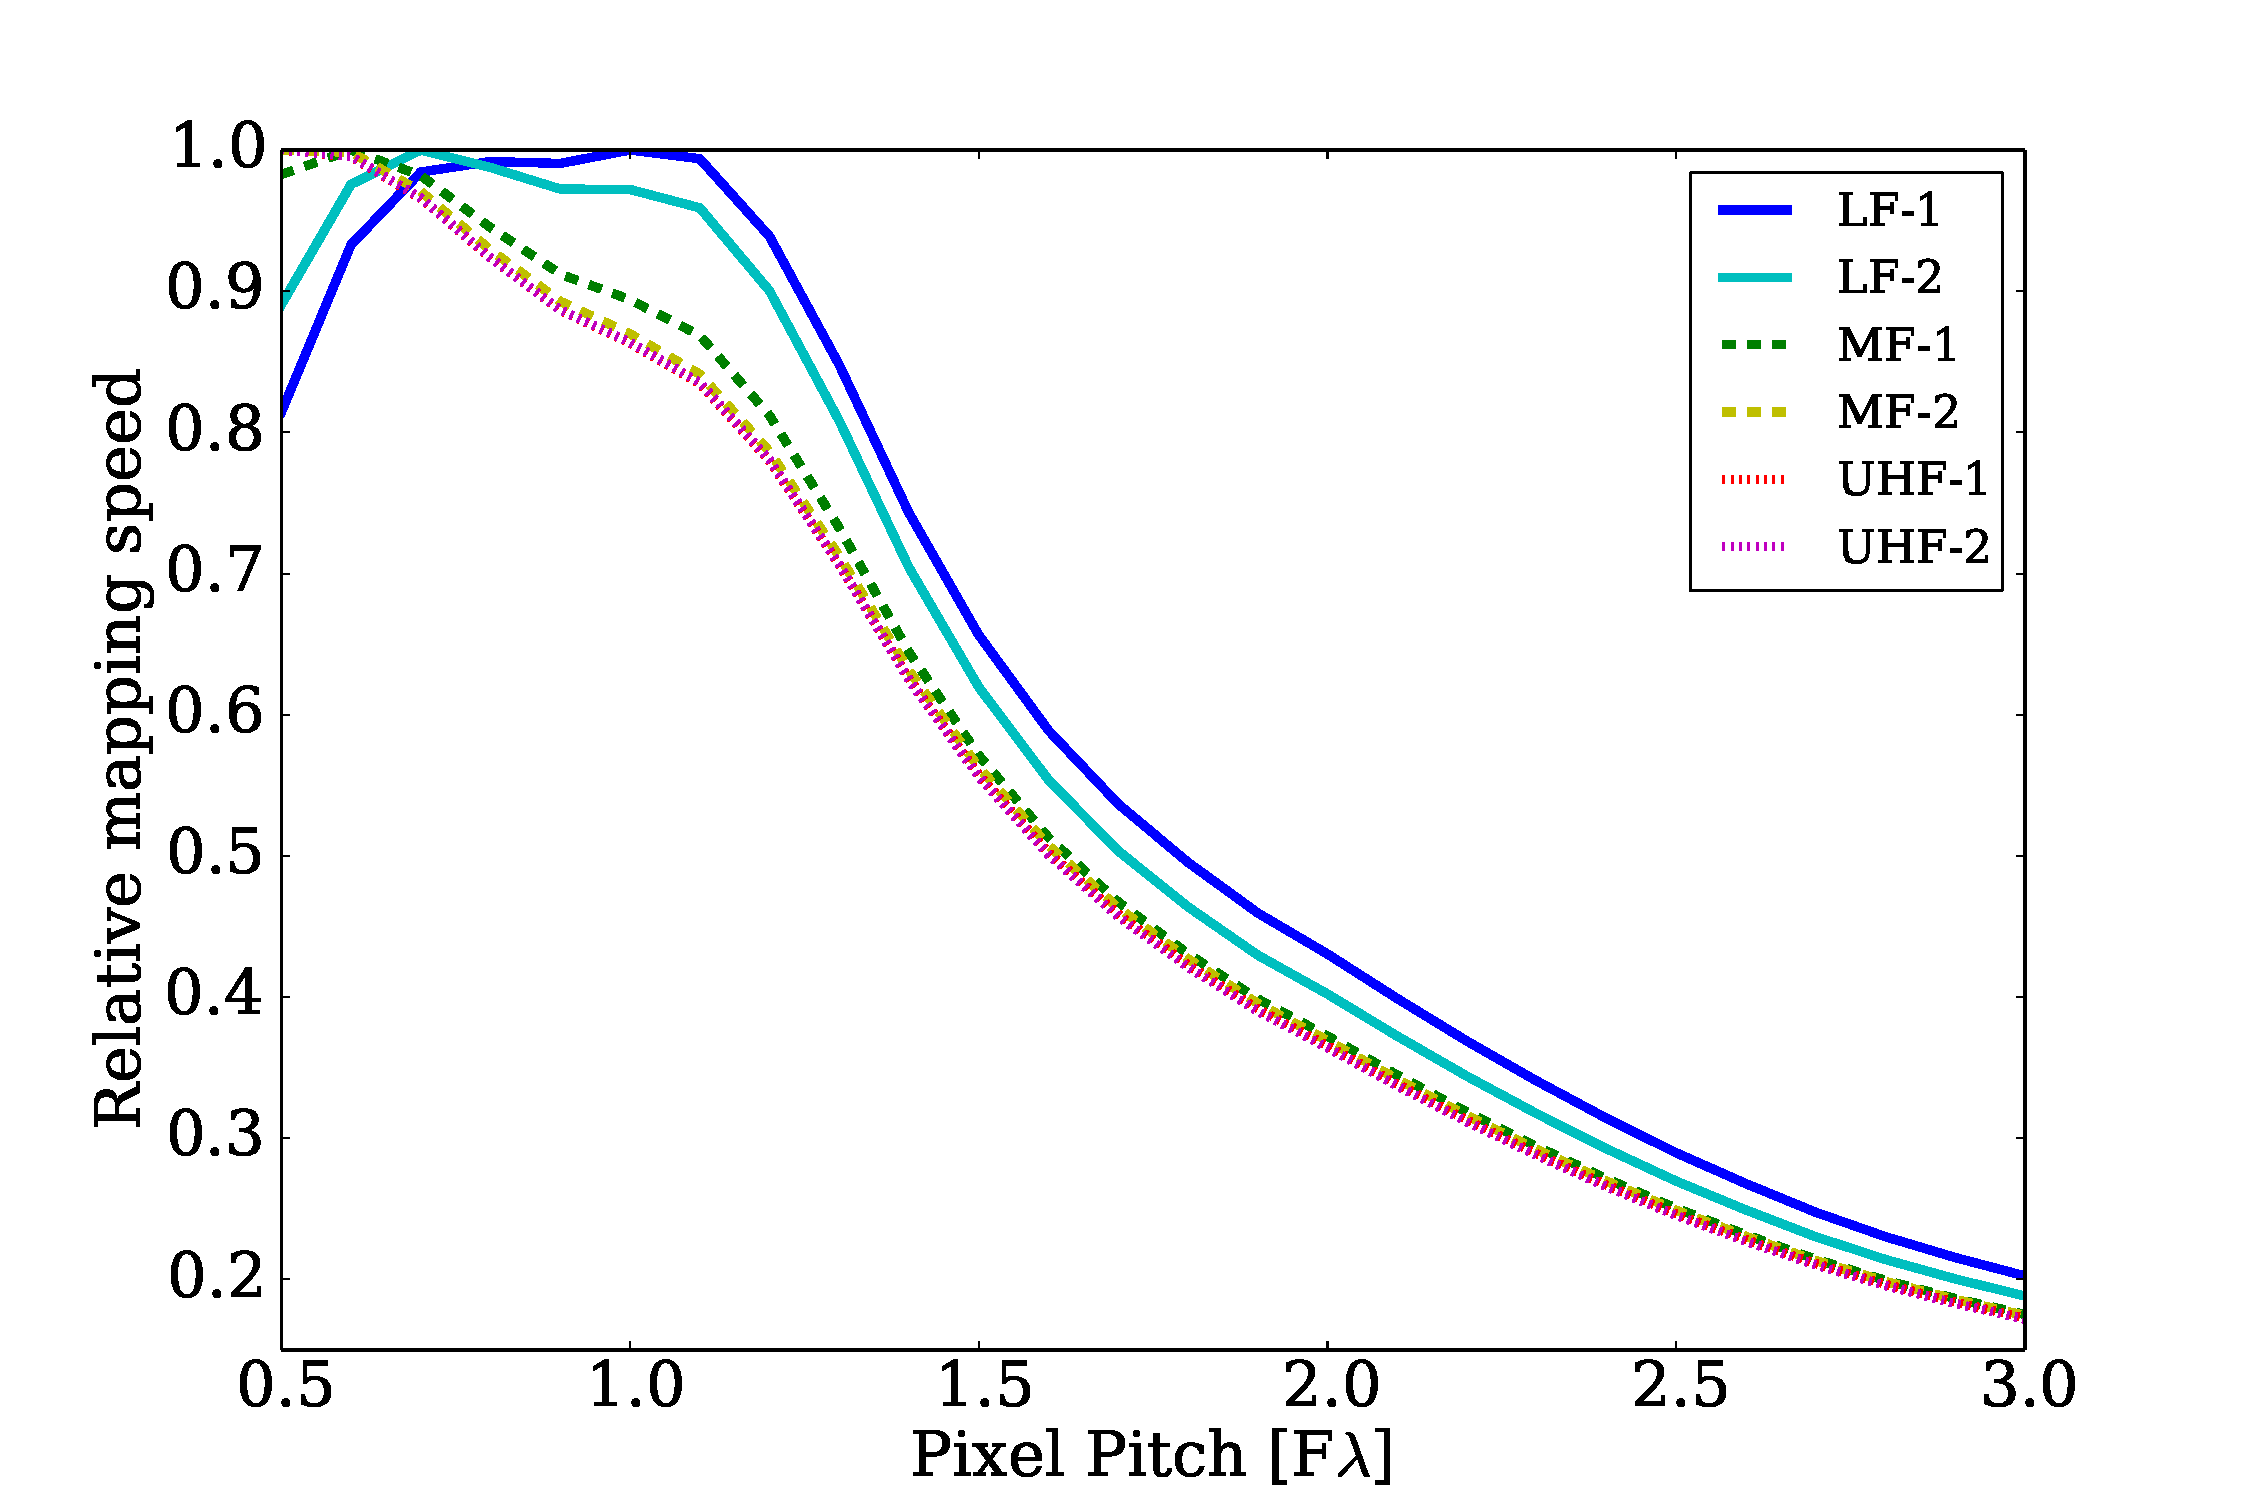
\includegraphics[width=0.48\linewidth]{SensitivityCalculator/Figures/MSvsPixelSize_LAT.pdf}
    }
    \subfloat[\label{fig:so_pix_size:b}]{
        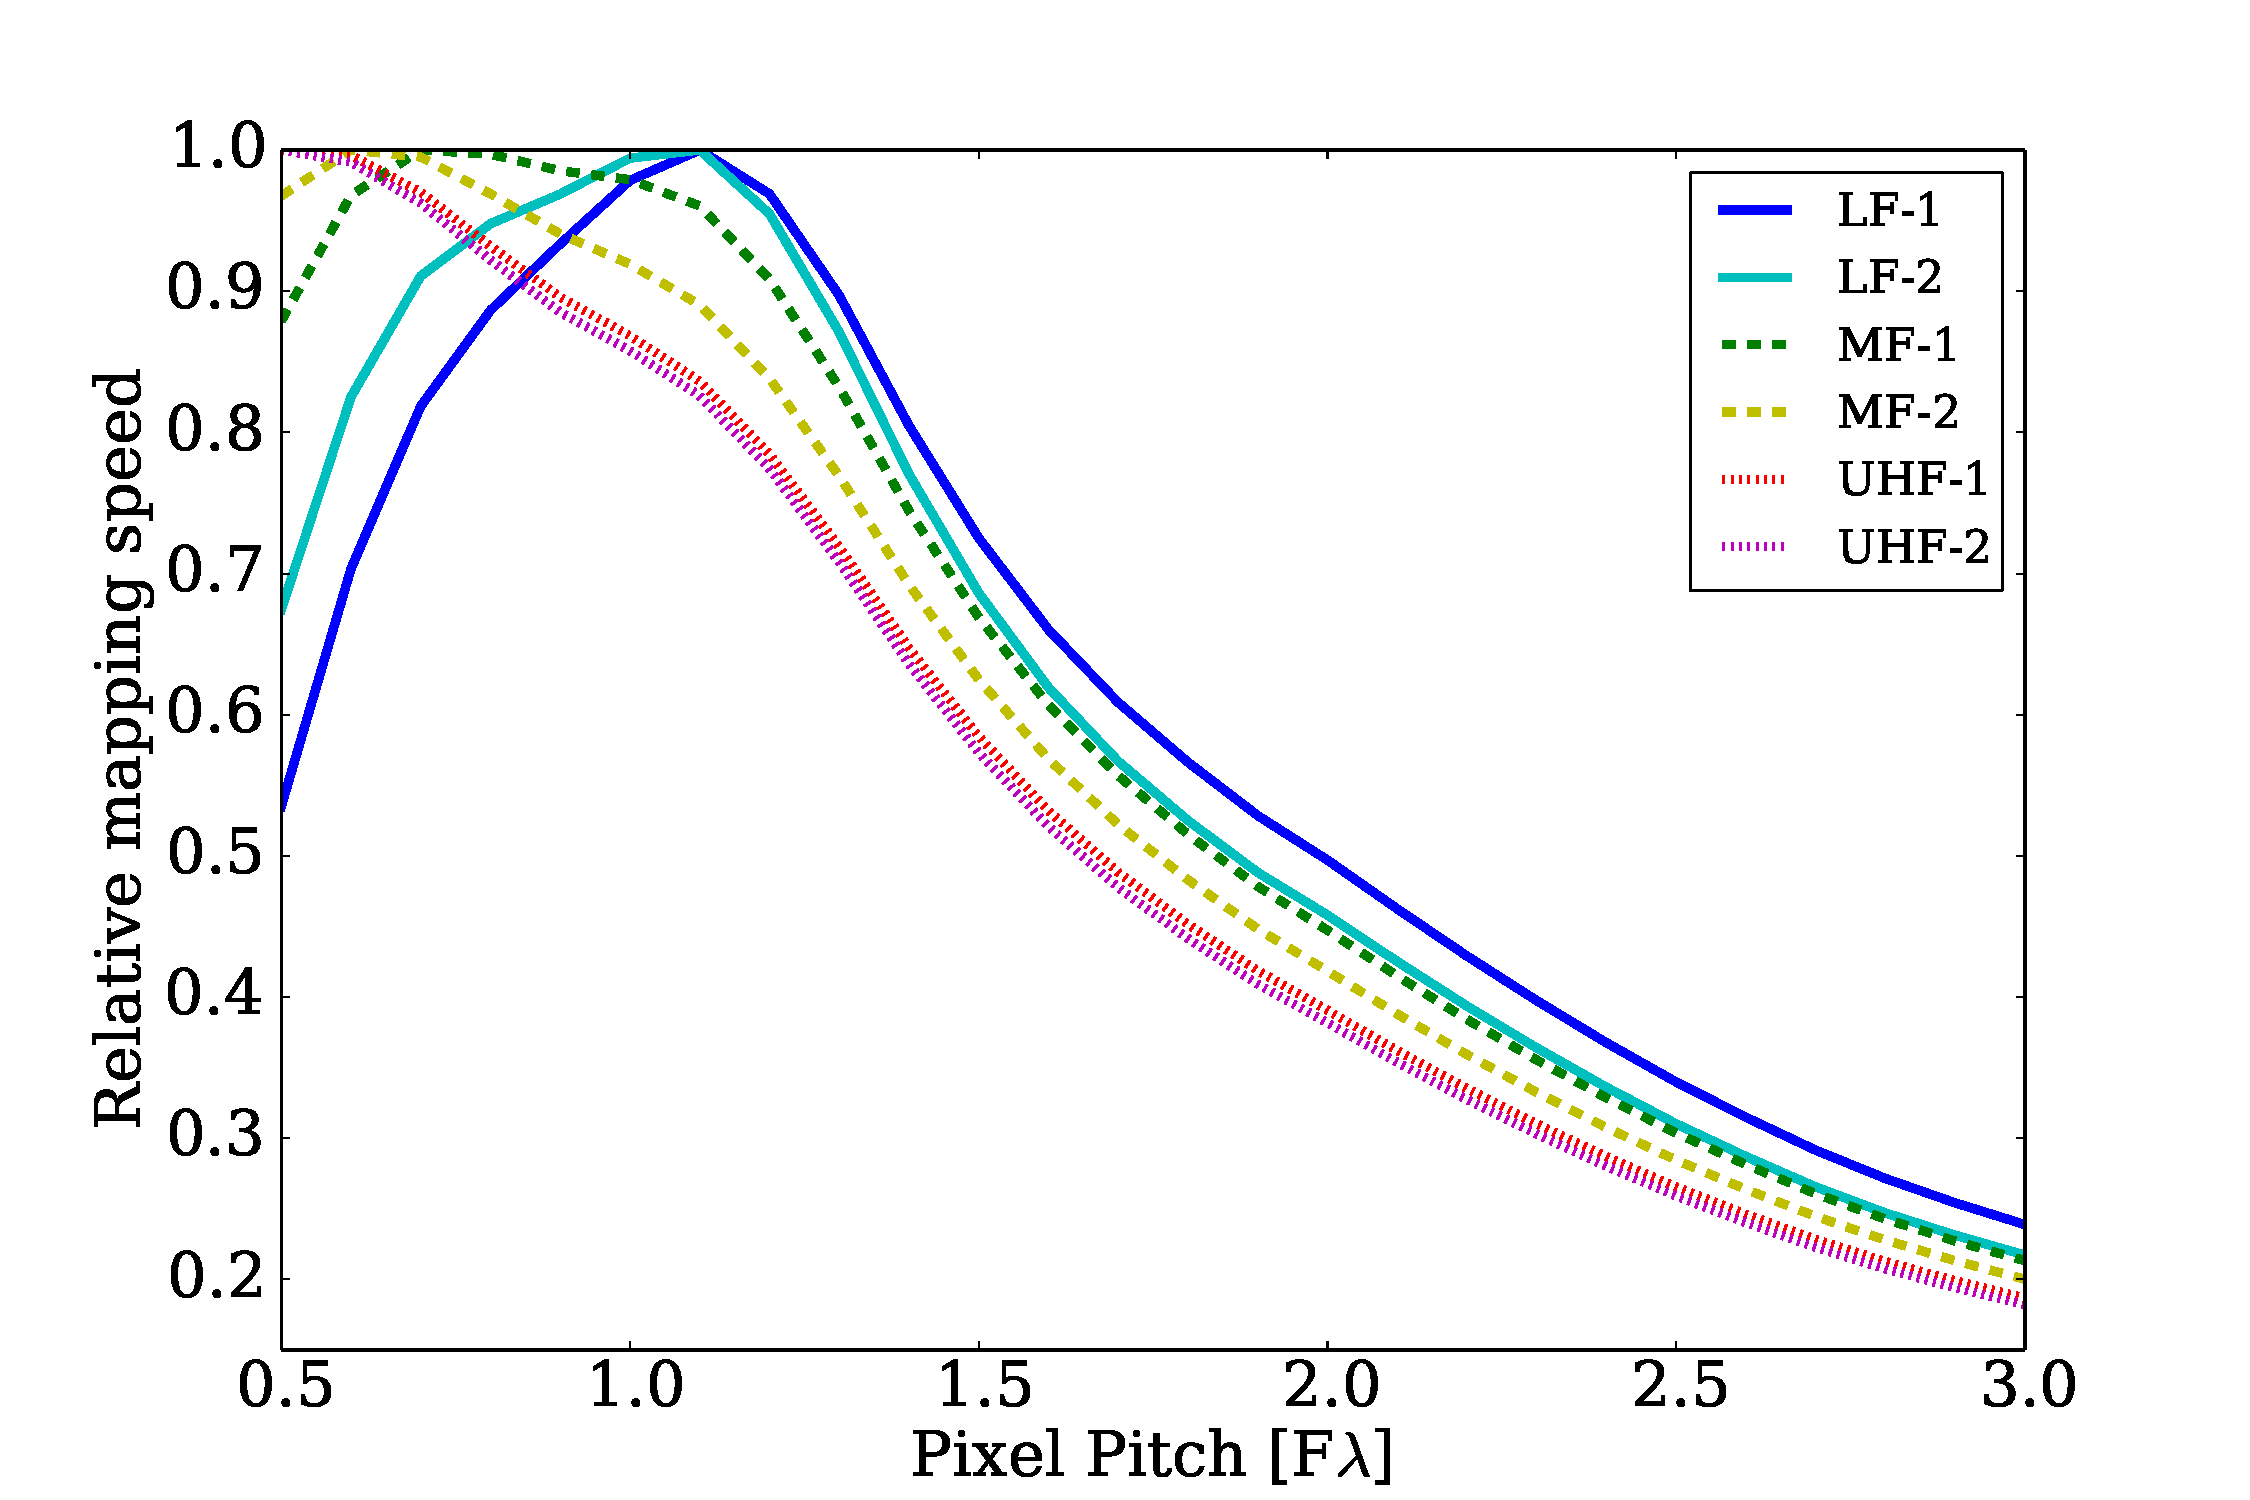
\includegraphics[width=0.48\linewidth]{SensitivityCalculator/Figures/MSvsPixelSize_SAC.pdf}
    }
    \caption[Sensitivity comparison between candidate SO LAT configurations]{Relative MS in each frequency band in the LAT (Fig.~\ref{fig:so_pix_size:a}) and SAT (Fig.~\ref{fig:so_pix_size:b}) against pixel pitch, plotted in units of $F \lambda$. Smaller pixels are favored until pitches $\sim$ 1.2~$F \lambda$, at which point the MS curve flattens due to detector-to-detector optical correlations. The curves for each frequency channel are individually peak-normalized.}
    \label{fig:so_pix_size}
\end{figure}

\begin{figure}[!ht]
    \subfloat[\label{fig:so_prim_spill:a}]{
        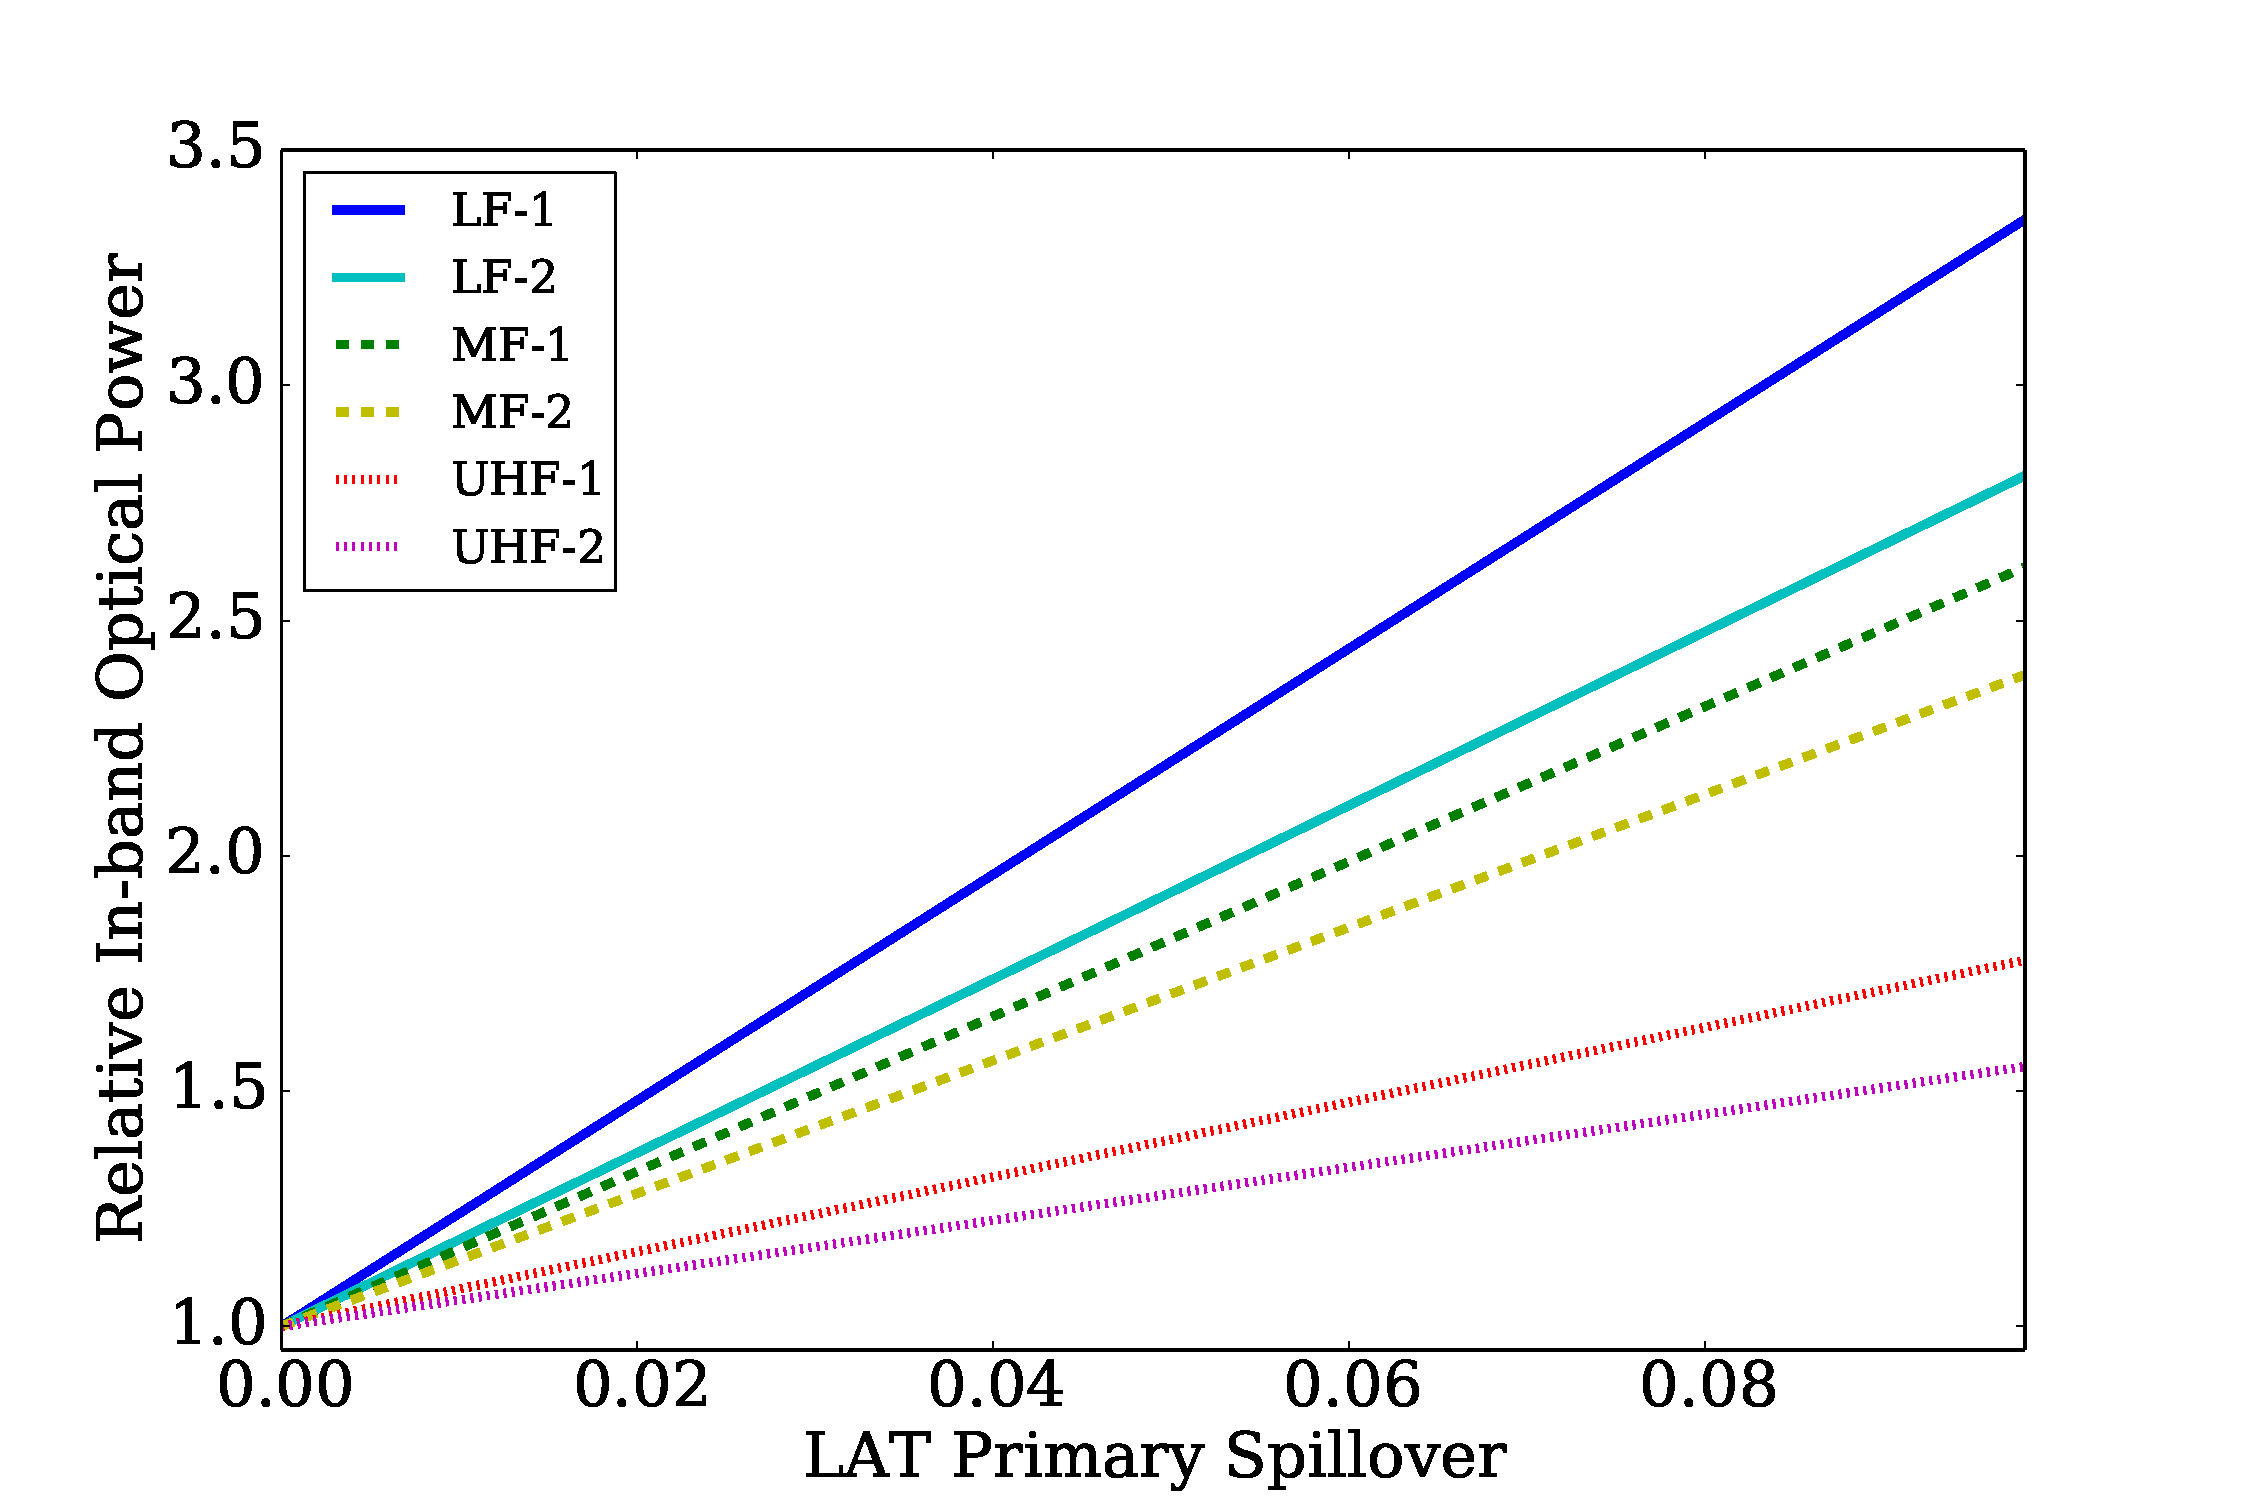
\includegraphics[width=0.48\linewidth]{SensitivityCalculator/Figures/POvsPrimSpill_LAT.pdf}
    }
    \subfloat[\label{fig:so_prim_spill:b}]{
        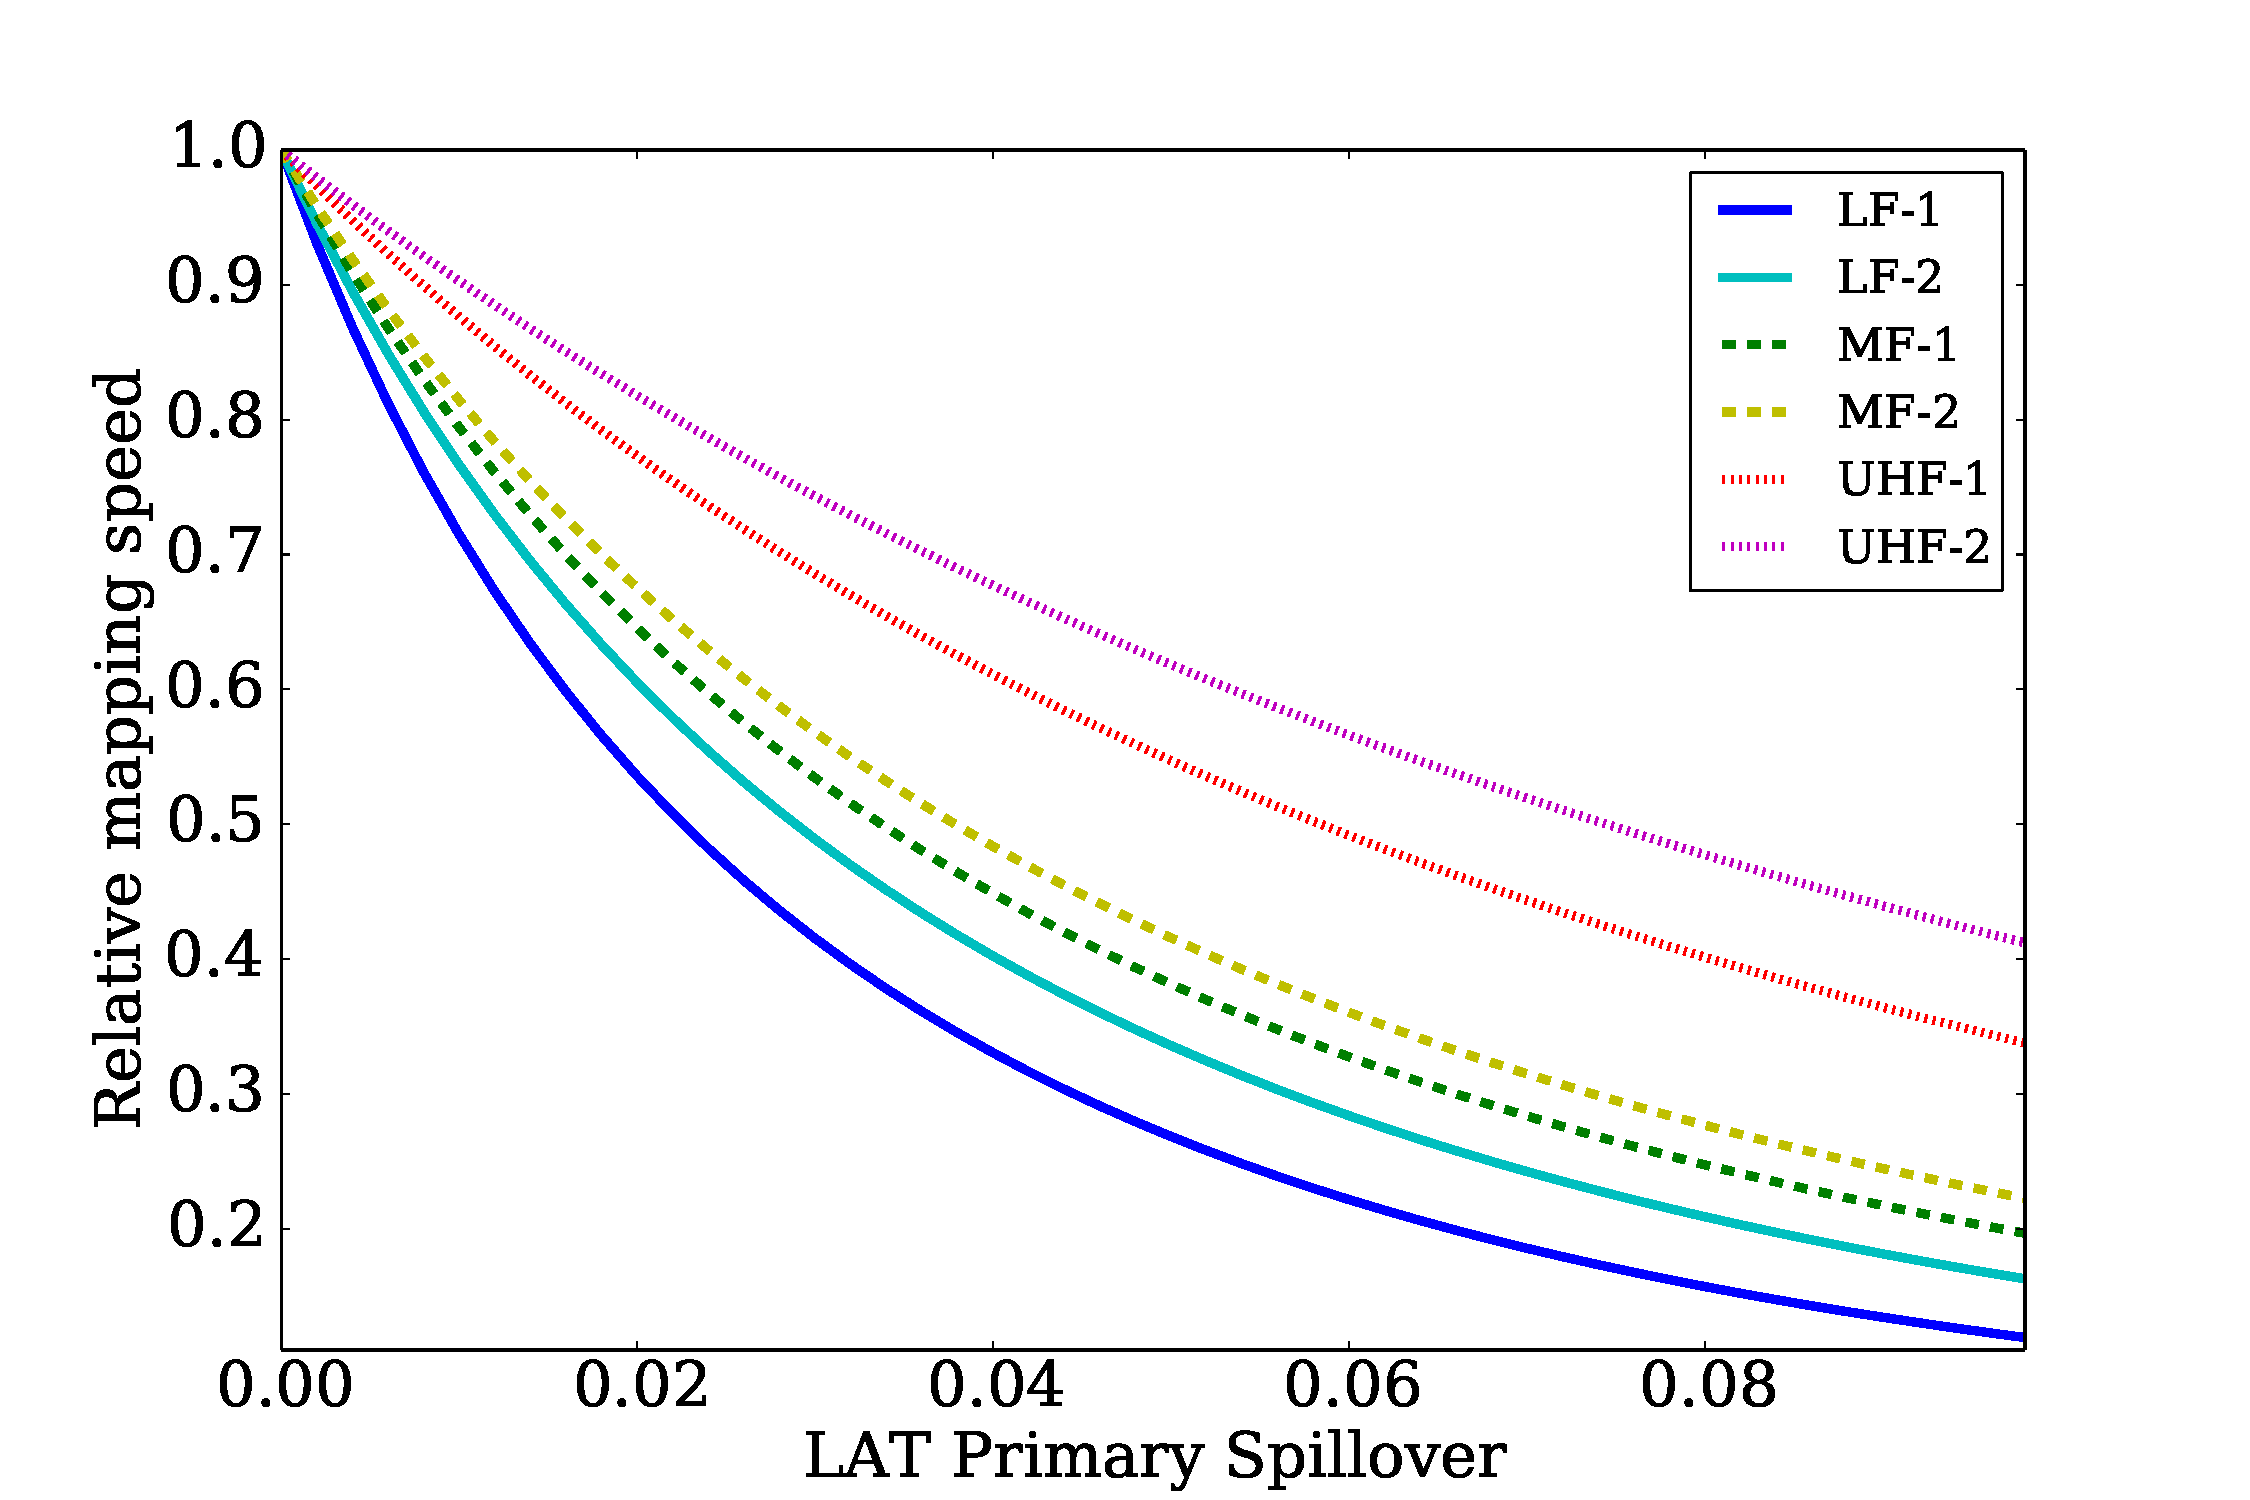
\includegraphics[width=0.48\linewidth]{SensitivityCalculator/Figures/MSvsPrimSpill_LAT.pdf}
    }
    \caption[Impact of SO LAT primary spillover on optical power and mapping speed]{The relative optical power (Fig.~\ref{fig:so_prim_spill:a}) and MS (Fig.~\ref{fig:so_prim_spill:b}) in each LAT frequency band vs. primary spillover fraction. Lower spillover is always better for sensitivity, but the MS impact is more pronounced at low frequencies. The curves for each frequency channel are individually peak-normalized.}
    \label{fig:so_prim_spill}
\end{figure}

\section{Observation strategy optimization}

\begin{figure}[!ht]
    \subfloat[\label{fig:so_ms_atm:a}]{
        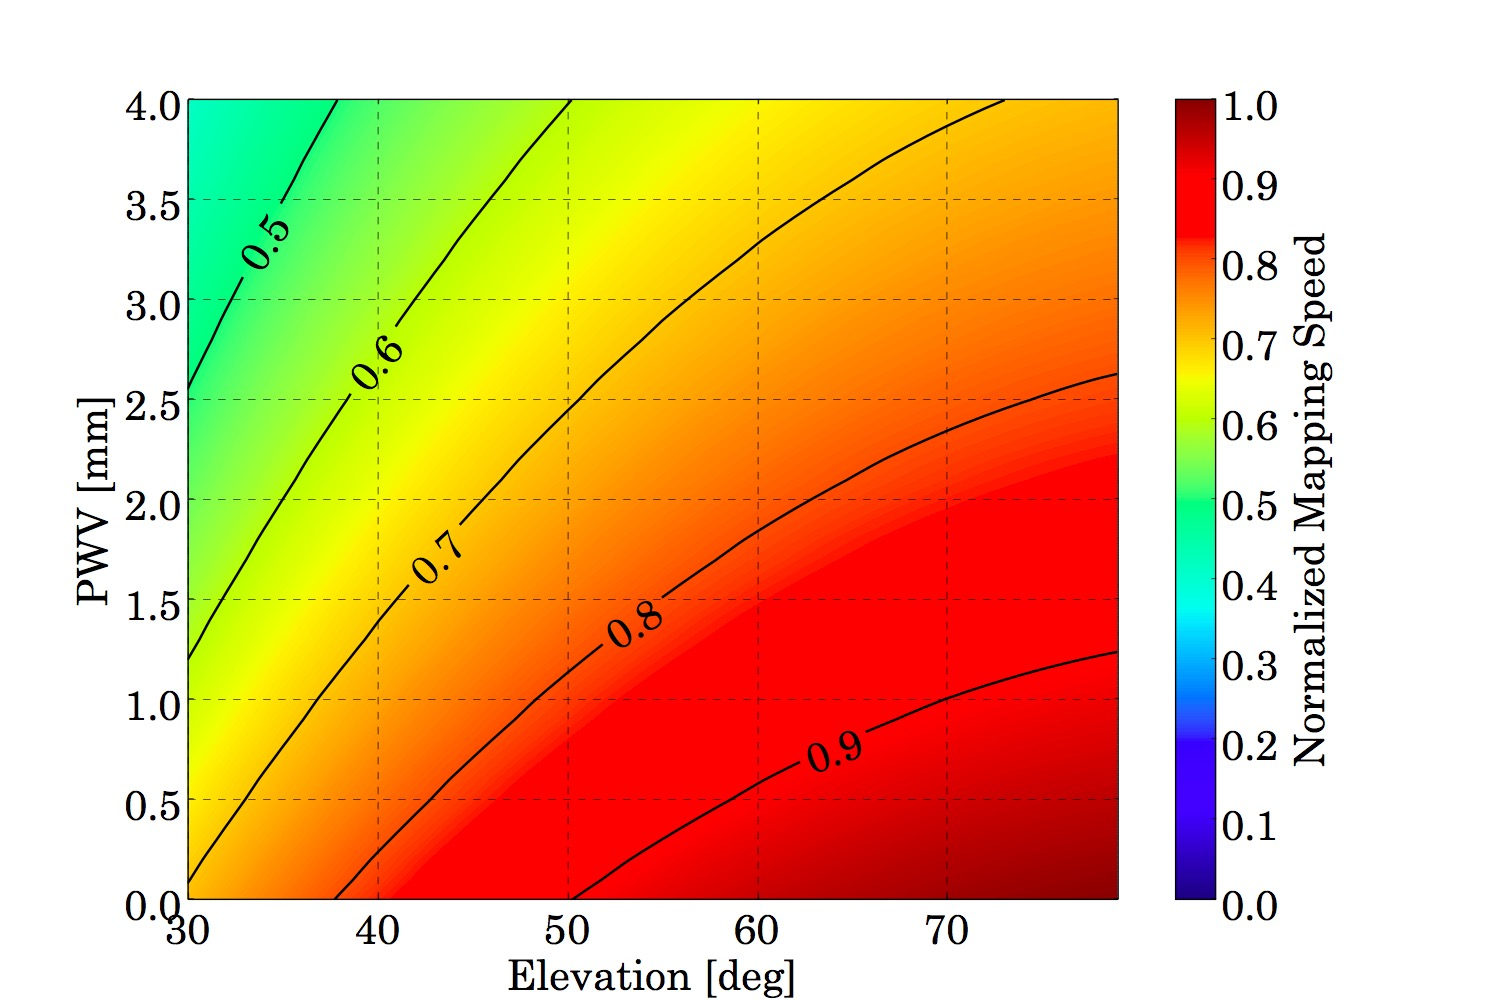
\includegraphics[width=0.48\linewidth]{SensitivityCalculator/Figures/MSvsATM_90.jpg}
    }
    \subfloat[\label{fig:so_ms_atm:b}]{
        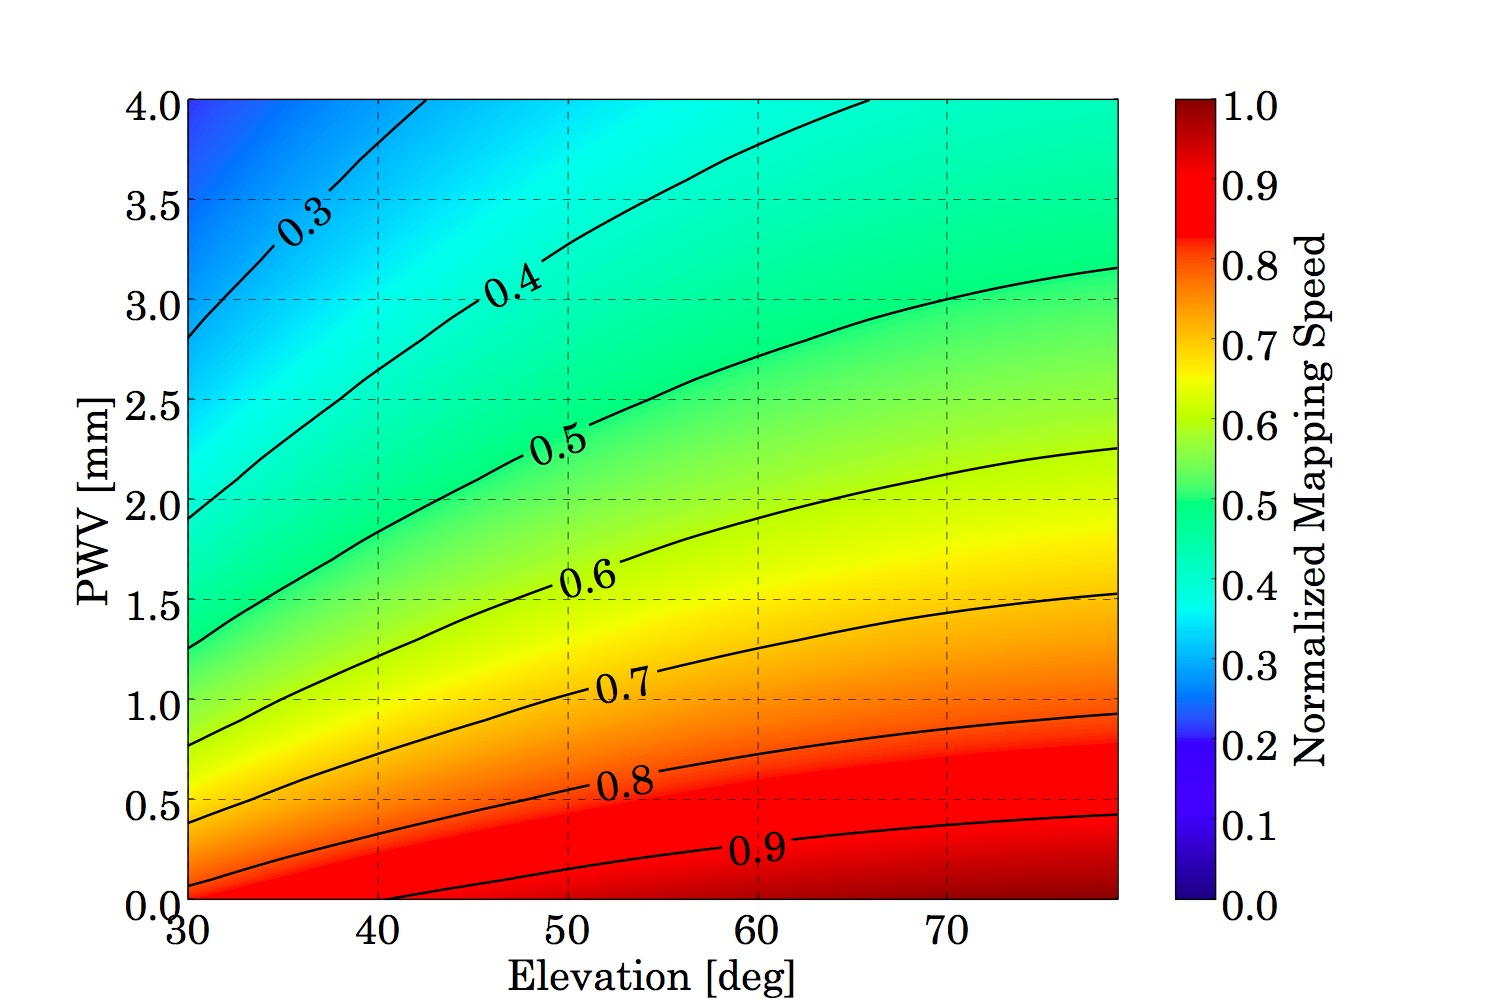
\includegraphics[width=0.48\linewidth]{SensitivityCalculator/Figures/MSvsATM_150.jpg}
    }
    \caption[Impact of boresight elevation and PWV on SO mapping speed]{Normalized MS vs. PWV and elevation at the Cerro Toco Atacama observation site in the 90 (Fig. \ref{fig:so_ms_atm:a}) and 150~GHz (Fig. \ref{fig:so_ms_atm:b}) bands in the LAT. The impact of elevation is more prominent in the low band, while the impact of water is more prominent in the high band. Additionally, the gradient of MS vs. sky conditions is larger at higher frequency. These tables are easy to generate using BoloCalc and are useful inputs to scan strategy optimization.}
    \label{fig:so_ms_atm}
\end{figure}

The ability to accurately and efficiently evaluate the sensitivity of varied instrument configurations is critical to providing rapid feedback to a project's designs. Therefore, BoloCalc is devised to be more broadly applicable, flexible, and detailed than its predecessors within \textsc{Polarbear} and ACT. In the following subsections, we outline the layout of the calculator, describe its input parameters, discuss how it calculates NEPs, and highlight a few of its state-of-the-art features.

\begin{table}[!ht]
	\centering
    \begin{minipage}[t]{0.45\textwidth}
    \centering
    \tabulinesep=0.8mm
	\begin{tabu}[t]{|| X[1,c] ||}
    \hline
    \textbf{Layer 1: foreground parameters} \\
    \hline
    \hline
    Synchrotron spectral index \\
    \hline
    Synchrotron amplitude \\
    \hline
    Dust spectral index \\
    \hline
    Dust effective blackbody temperature \\
    \hline
    Dust pivot frequency \\
    \hline
    Dust amplitude \\
    \hline
    \end{tabu}
    \end{minipage}
    \begin{minipage}[t]{0.45\textwidth}
    \tabulinesep=0.8mm
    \begin{tabu}[t]{|| X[1,c] ||}
    \hline
    \textbf{Layer 2: atmosphere and telescope parameters} \\
    \hline
    \hline
    Observation site \\
    \hline
    PWV (distribution) \\
    \hline
    Observation time \\
    \hline
    Sky fraction \\
    \hline
    Observation efficiency \\
    \hline
    NET margin \\
    \hline
    Boresight elevation (distribution) \\
    \hline
    \end{tabu}
    \end{minipage}
    \begin{minipage}[t]{0.45\textwidth}
    \centering
    \vspace{2mm}
    \tabulinesep=0.8mm
    \begin{tabu}[t]{|| X[1,c] | X[1,c] ||}
    \hline
    \multicolumn{2}{|| c ||}{\textbf{Layer 3: camera parameters}} \\
	\hline
    \hline
    \multicolumn{2}{|| c ||}{Boresight elevation} \\
    \hline
    \multicolumn{2}{|| c ||}{Pixel elevation distribution} \\
    \hline
    F-number at the focal plane & Focal plane temperature \\
    \hline
    \multicolumn{2}{|| c ||}{\textit{Optical element definitions}} \\
    \hline
    Temperature & Absorption \\
    \hline
    \multicolumn{2}{|| c ||}{Aperture stop spillover efficiency} \\
    \hline
    Reflection & Thickness \\
    \hline
    Index & Loss tangent \\
    \hline
    Conductivity & Surface roughness \\
    \hline
    Spillover fraction & Spillover temperature \\
    \hline
    Scattering fraction & Scattering temperature \\
    \hline
    \end{tabu}
    \end{minipage}
	\begin{minipage}[t]{0.45\textwidth}
    \centering
    \vspace{2mm}
    \tabulinesep=0.8mm
    \begin{tabu}[t]{|| X[1,c] | X[1,c] ||}
    \hline
    \multicolumn{2}{|| c ||}{\textbf{Layer 4: detector parameters}} \\
    \hline
    \hline
    Band center & Fractional bandwidth \\
    \hline
    Pixel size & Number of detectors per wafer \\
    \hline	
    Number of wafers per camera & Pixel beam waist \\
    \hline
    Optical efficiency & Saturation power \\
    \hline
    Ratio of saturation power to optical power & Bolometer operating temperature \\
    \hline
    Thermal carrier index & $F_{\mathrm{link}}$ \\
    \hline
    Ratio of operating temperature to bath temperature & Ratio of readout NEP to total NEP \\
    \hline
    Bolometer resistance & SQUID NEI \\
    \hline
    \multicolumn{2}{|| c ||}{Yield} \\
    \hline
    \end{tabu}
    \end{minipage}
    \vspace{1mm}
    \caption{User-defined parameters within a BoloCalc project. Each of the ``\textit{Optical element definitions}'' are defined for every optical element, except for the aperture spill efficiency, which is only defined for the cold stop.}
    \label{tab:bolocalc_input_parameters}
\end{table}

BoloCalc implements several features that are upgrades to its predecessor calculators within ACT and \textsc{Polarbear}. These features improve instrument modeling and increase the accuracy of NET estimates, allowing for better-informed instrument design decisions.

A list of input parameters for each layer is shown in Table~\ref{tab:bolocalc_input_parameters}.

\section{Graphical user interface}

\begin{figure}[!ht]
    \centering
    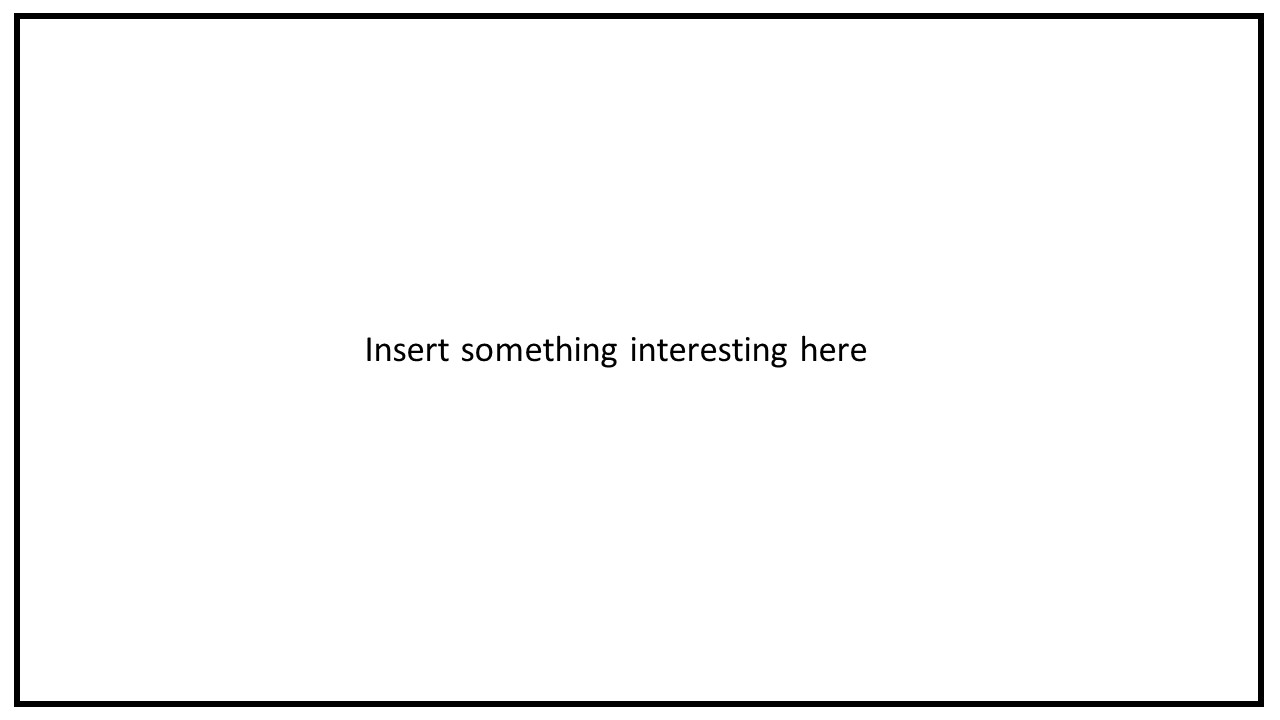
\includegraphics[width=0.98\linewidth]{Other/empty.jpg}
    \caption[Snapshot of the BoloCalc graphical user interface]{Snapshot of the BoloCalc graphical user interface}
    \label{fig:bolocalc_gui}
\end{figure}

BoloCalc can estimate the uncertainty in NET as a function of the uncertainty in low-level instrument parameters. Every parameter in BoloCalc accepts a central value and standard deviation, and every optical element and detector band can have error bars on its input spectrum. The resulting NET distribution is determined by independently sampling each parameter using the Monte Carlo method over a user-defined number of iterations. 

This functionality is particularly useful when importing measurements with statistical and/or systematic errors, as BoloCalc can assess an experiment's progression from an abstract design to a real system. Typical uncertainties include variation of detector parameters across a fabricated array, errors in the measurements of optical and RF filter bands, and variation of filter and lens temperatures across multiple cooldowns. The ability to propagate low-level parameter errors to NET is important to both understand the impact an isolated measurement on overall instrument performance and properly handle the interconnection of measured subsystems in a complex instrument.

BoloCalc is equipped to handle realistic filter functions. Unlike top hats, realistic filter functions do not display a perfectly vertical drop to zero at the band edges and include ripples in power originating from on-chip dielectric filters and resonances in anti-reflection coatings. BoloCalc's filter function module accepts measured and simulated bands, providing insight into the effect of various realistic bands on sensitivity. The module also enables optimization of the detector and coupling optics design. Filter optimization is discussed further in Sec.~\ref{sec:Obs_band}.

In the following subsections, we highlight some of the most prominent ways that BoloCalc has been used to inform the SO design.

In addition to generating MS contours, BoloCalc can import histograms of pixel elevation with respect to camera boresight. This capability is particularly useful for the SAT, which has a large FOV and therefore is expected to have a large instantaneous variation in optical power across the focal plane. BoloCalc also accepts histograms of PWV values, which allows it to calculate NET variations caused by varied observing conditions.

Lower $P_{\mathrm{sat}}$ leads to lower MS but also lower $\eta_{\mathrm{obs}}$, as the detectors will saturate at lower $T_{\mathrm{sky}}$.  

With increasing optical load comes increasing photon noise and therefore decreasing mapping speed. Additionally, with increasing $P_{\mathrm{sat}}$ comes increasing thermal carrier and readout noise, which decreases mapping speed further. However, being able to handle increasing $T_{\mathrm{sky}}$

\begin{figure}[!ht]
    \subfloat[\label{fig:pb2c_popt_hist:a}]{
        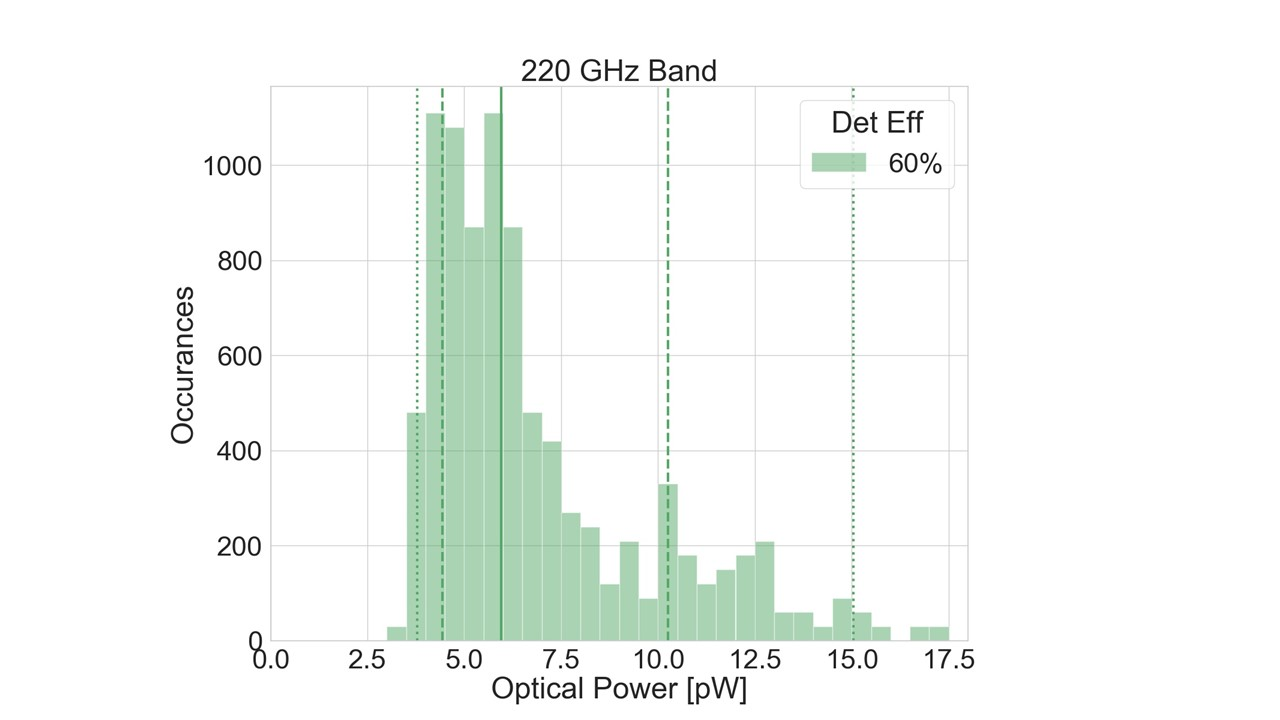
\includegraphics[width=0.48\linewidth]{BoloCalc/Figures/pb2c_220_popt_hist.jpg}
    }
    \subfloat[\label{fig:pb2c_popt_hist:b}]{
        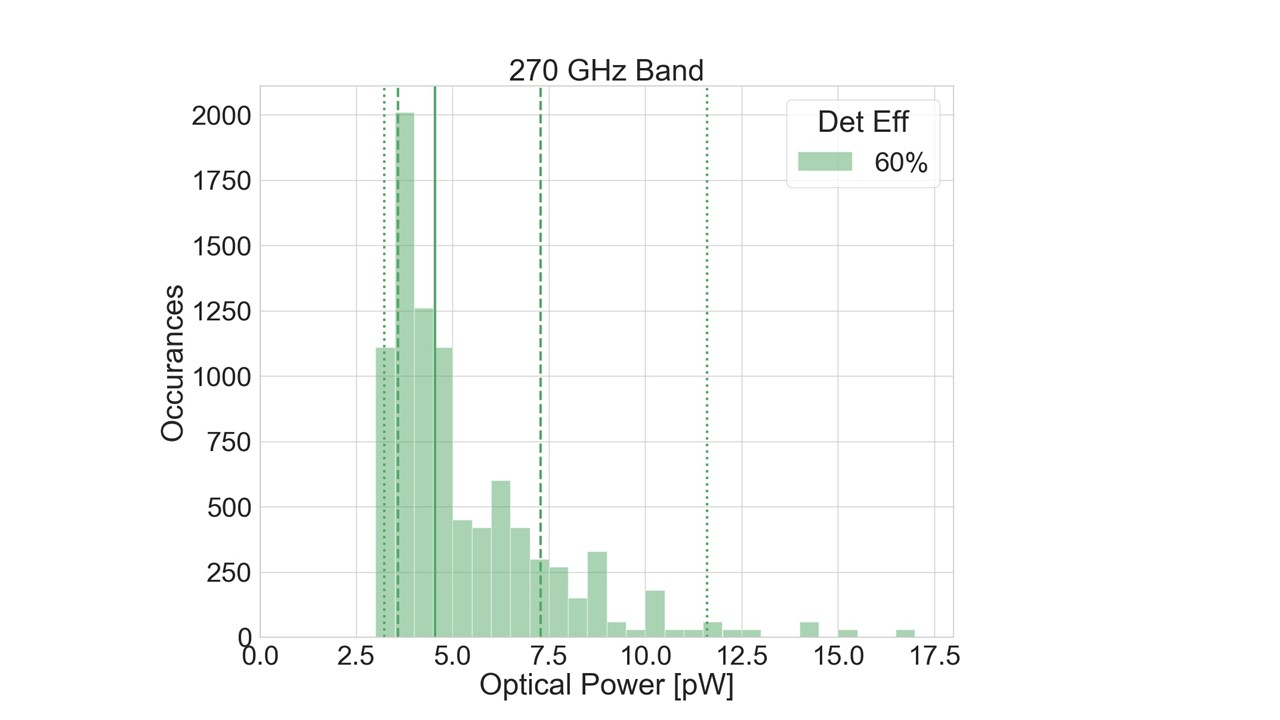
\includegraphics[width=0.48\linewidth]{BoloCalc/Figures/pb2c_270_popt_hist.jpg}
    }
    \caption[Expected optical power for PB2c in both the 220 and 270 GHz bands as simulated by BoloCalc]{\ref{fig:pb2c_popt_hist:a} shows a historgram of the expected optical power in the 220 GHz band on PB2c given undertainties in dewar temperature, sky power, and detector bandpass, assuming a detector efficiency of 60\%. \ref{fig:pb2c_popt_hist:b} shows the same histogram but for the 270 GHz band. The solid line denotes the median, and the dashed and dotted lines represent the 68\% and 95\% confidence levels, respectively. These plots demonstrate BoloCalc's ability to fold uncertainties in instrument parameters into the expected measured values.}
    \label{fig:pb2c_popt_hist}
\end{figure}

\begin{figure}[!t]
    \subfloat[\label{fig:pb2c_psat_ms:a}]{
        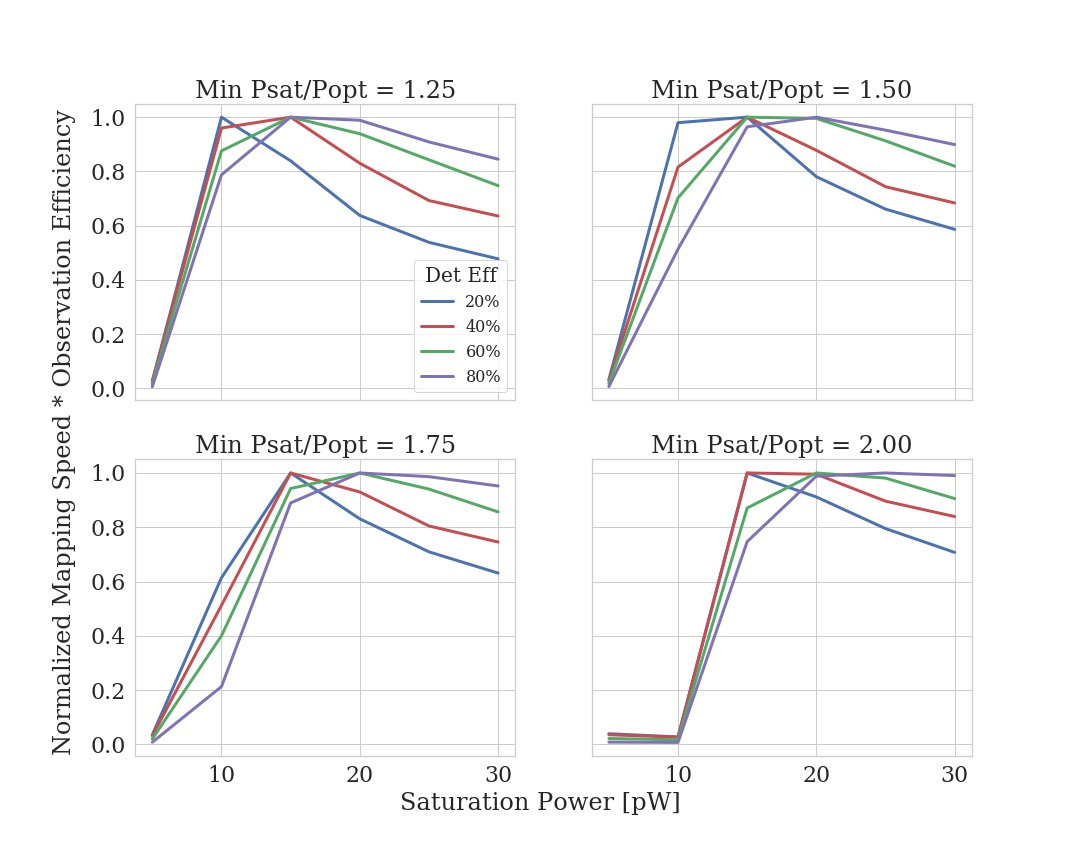
\includegraphics[width=0.48\linewidth]{BoloCalc/Figures/220_Psat_MS_obsEff_allEffs_1.jpg}}
    \subfloat[\label{fig:pb2c_psat_ms:b}]{
        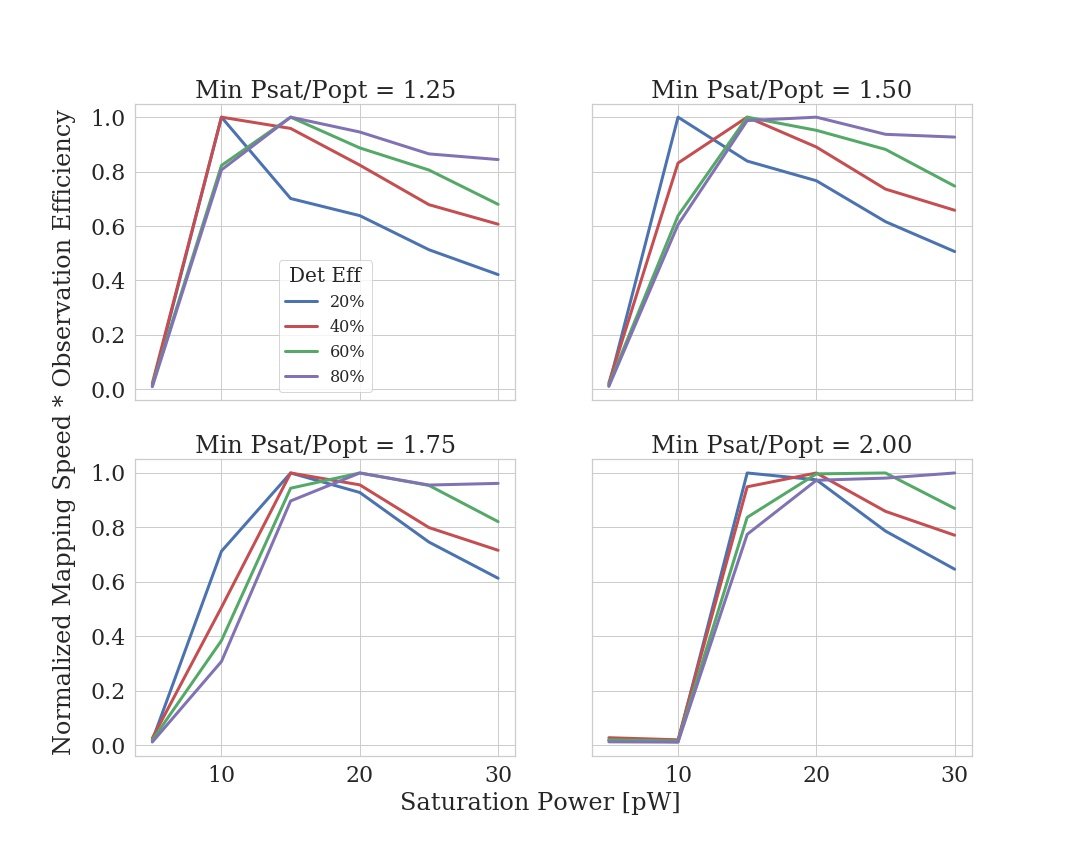
\includegraphics[width=0.48\linewidth]{BoloCalc/Figures/270_Psat_MS_obsEff_allEffs_1.jpg}}
    \caption[Impact of PB2c Psat on mapping speed for various detector efficiencies and minimum allowed value of Pelec/Popt]{\ref{fig:pb2c_psat_ms:a} shows the impact of saturation power on mapping speed in the 220 GHz band for various values of detector efficiency and minimum allowed Pelec/Popt. \ref{fig:pb2c_psat_ms:b} shows the same plot for the 270 GHz band.}
    \label{fig:pb2c_psat_ms}
\end{figure}